\documentclass[journal,12pt,twocolumn]{IEEEtran}
\usepackage{amsmath,amssymb,amsfonts,amsthm}
\usepackage{txfonts}
\usepackage{tkz-euclide}
\usepackage{listings}
\usepackage{gvv}
\usepackage[latin1]{inputenc}
\usepackage{array}
\usepackage{pgf}
\usepackage{lmodern}

\begin{document}
\bibliographystyle{IEEEtran}

\vspace{3cm}

\title{}
\author{EE23BTECH11217 - Prajwal M$^{*}$
}
\maketitle
\newpage
\bigskip

% \renewcommand{\thefigure}{\theenumi}
% \renewcommand{\thetable}{\theenumi}


\section*{Exercise 9.1}

\noindent \textbf{12} \hspace{2pt}Write the five terms at n = 1, 2, 3, 4, 5 of the sequence and obtain the corresponding series

$ x \brak{n} =
\begin{cases}
-1 & n = 0 \\
\frac{x \brak{n-1}}{n} & n > 0\\
	0 & n < 0
\end{cases}
$
\\

\noindent Solution:

\noindent
\begin{align}
	x \brak{1} & = \frac{x \brak{0}}{1} = -1 \\
x \brak{2} & = \frac{x \brak{1}}{2} = -\frac{1}{2} \\
x \brak{3} & = \frac{x \brak{2}}{3} = -\frac{1}{2   3} = -\frac{1}{6}\\
x \brak{4} & = \frac{x \brak{3}}{4} = -\frac{1}{2   3   4} = -\frac{1}{24}\\
x \brak{5} & = \frac{x \brak{4}}{5} = -\frac{1}{2   3   4   5} = -\frac{1}{120}
\end{align} \\

% So the first five terms of the series are:
% $$-1 , -\frac{1}{2}, -\frac{1}{6}, -\frac{1}{24},  -\frac{1}{120}$$ \\

The corresponding series:
\begin{align}
	\sum_{n=-\infty}^{\infty} x \brak{n} & = \ldots + 0 + x\brak{0} + x \brak{1} + x \brak{2} + \ldots \\
	& = \ldots + 0 + \brak{-1} +  \brak{-1} +   \brak{-\frac{1}{2} } + \ldots 
\end{align}

The nth term of the series is,
\begin{align}
    x \brak{n} & = \frac{-1}{n!}  \brak{u \brak{n}}
\end{align}

\begin{figure}
  \centering
  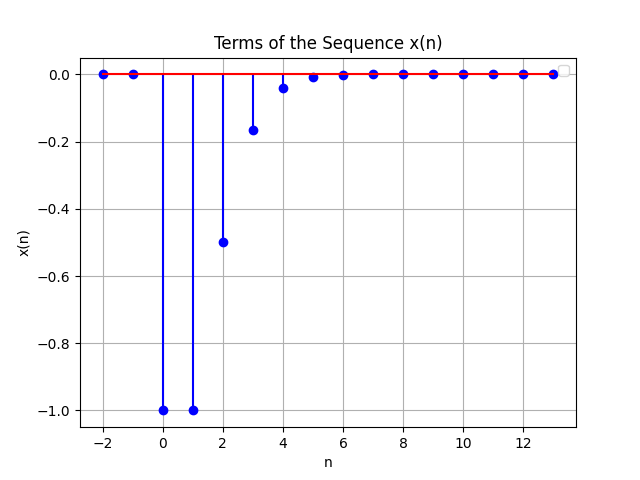
\includegraphics[width=0.5\textwidth]{figs/plot.png}
\end{figure}

The Z-transform of $ x \brak{n} $ is given by:
\begin{align}
	x \brak{n} \ztransform X \brak{z} 
\end{align}

\begin{align}
    X \brak{z} & = \sum_{n=-\infty}^{\infty} x \brak{n}   z^{-n} \\
    & = \sum_{n=-\infty}^{\infty} \frac{-1}{n!}  u \brak{n}   z^{-n} \\
    & = \sum_{n=0}^{\infty} \frac{-1}{n!}   z^{-n} \\
    & = - e^{z^{-1}}
\end{align}

So, the Z-transform of the given series is
$ - e^{z^{-1}} $.\\

For the series to converge, the ratio test must be satisfied for n $\geq$ 0
\begin{align}
 \lim_{{n \to \infty}}  \left| \frac{x \brak{n+1} z^{- \brak{n+1}}}{x \brak{n} z^{-n}}  \right| & <  1 \\
\lim_{{n \to \infty}}  \left| \frac{-z^{-n-1} n!}{-z^{-n}  \brak{n+1}!} \right| & < 1\\
\lim_{{n \to \infty}}  \left| \frac{z^{-1}}{n+1}  \right| & < 1
\end{align}

The condition is satisfied for $ z \neq 0 $ \\

Hence, ROC of Z transform is 
\begin{align}
	z\in\mathbb{C} : z \neq 0.
\end{align}
\begin{table}[h]
  \centering
  \begin{tabular}{|c|c|}
    \hline
    	\textbf{Symbol} & \textbf{Parameters} \\
    \hline
	  x(n) & general term of the series \\
    \hline
	  $X$(z) & Z-transform of x(n) \\
    \hline 
	  u(n) & unit step function \\
    \hline

  \end{tabular}
  \vspace{0.3cm}
  \caption{Parameters}
  \label{tab:parameters}
\end{table}


\end{document}
